\documentclass[unicode,12pt]{beamer}
\usetheme[progressbar=frametitle]{metropolis}    %プレゼンのテーマ設定

%if want to use pdfLatex, specify \iffalse to preamble for LuaLatex and XeLatex
%--------------- preamble for LuaLatex ------------------%

\iffalse
\usepackage{luatexja}
\usepackage[ipaex]{luatexja-preset}
\renewcommand{\kanjifamilydefault}{\gtdefault}
\setsansfont{Calibri}
\fi

%-----------------------------------------------------%

%--------------- preamble for XeLatex -------------------%

\iftrue
\usepackage{xltxtra}
\XeTeXlinebreaklocale "ja"
\usepackage{zxjatype}
\setCJKmainfont[]{Meiryo}
\setsansfont[Scale = 1.1]{Calibri}  % or Arial (Scale = 1)
\fi

%-----------------------------------------------------%

%--------------- general preamble -----------------------%

\definecolor{Cerulean blue}{rgb}{0.16, 0.32, 0.75}
\definecolor{darkcerulean}{rgb}{0.03, 0.27, 0.49}
\definecolor{skyblue}{rgb}{0.4, 0.6, 1.0}
\definecolor{lightpink}{rgb}{1.0, 0.8, 0.76}  %for block color
\definecolor{gray}{gray}{0.8}

\setbeamertemplate{blocks}[default] % Blockの影を消す
%\setbeamertemplate{items}[default] % 箇条書きをシンプルに
\setbeamertemplate{navigation symbols}{} % ナビゲーションシンボルを消す
\setbeamertemplate{footline}[frame number] % フッターはスライド番号のみ
\setbeamertemplate{itemize item}[circle]
\setbeamertemplate{itemize subitem}{--}
\setbeamercolor{frametitle}{bg=skyblue} %or Cerulean blue
\setbeamercolor{title}{fg=darkcerulean}

\iffalse
\usebackgroundtemplate{
    \includegraphics[width=\paperwidth,height=\paperheight]{beamer_background1.pdf}
}
\fi

\usepackage{color}


\newcommand{\emphasis}[2][red]{{\bf{\color{#1} #2}}}
\newcommand{\caveat}[2][blue]{{\bf{\color{#1} #2}}}
\newcommand{\fpartial}[3][\partial]{\frac{#1 #2}{#1 #3}}
\newcommand{\hpartial}[4][\partial]{\frac{#1^{#2} #3}{#1 #4^{#2}}}

\newcommand{\dlinecell}[1]{\begin{tabular}{@{}c@{}} #1 \end{tabular}}

\def\argmax{\text{arg} \max}
\def\argmin{\text{arg} \min}

%-----------------------------------------------------%

\title{Seeds to succeed? Sequential giving to public projects}
\subtitle{Literature Review Workshop in 2020}
\author{Hiroki Kato}
\date{June 4, 2020}

\begin{document}

    \maketitle

    \section{Introduction}

    \begin{frame}
        \frametitle{}

        \centerline{
\includegraphics[width = 1.0\linewidth]{./0605kato_fig/crowdfunding2.PNG}}
        
    \end{frame}

    \begin{frame}
        \frametitle{Rule of Thumb of Fundraising}
    
        \begin{itemize}
            \item A common practice of fundraising: past contributions are announced to future donors.
            \item Varian (1994): The sequential provision enables the initial donor to free ride off subsequent donors because one donor's contribution is a perfect substitute for that of another. 
        \end{itemize}
        Thus, standard public goods theory cannot rationalize a rule of thumb of fundraising.
    
    \end{frame}

    \begin{frame}
        \frametitle{Andreoni's Insight}
    
        Andreoni (1998) shows that a sequential fundraising strategy is preferable when there are fixed production costs.
        \begin{itemize}
            \item Under the existence of fixed costs, simultaneous provision generates zero provision equilibrium. However, sequential provision overcomes this coordination failure.
            \item Evidence of a field experiment (List and Lucking-Reiley, 2002)
            \item But, this evidence cannot eliminate the predictions made by other models.
        \end{itemize}
    
    \end{frame}

    \begin{frame}
        \frametitle{What This Paper Did}
    
        Use lab experiments to examine the coordinating role of sequential giving in the presence and absence of fixed costs.
        \begin{itemize}
            \item RQ1: Do sequential moves increase giving when there are no fixed costs?
            \item RQ2: Do fixed costs give rise to inefficient outcomes under simultaneous provision?
            \item RQ3: If such inefficient outcomes exist, does sequential play help eliminate these inefficiencies and increase the likelihood of providing the public good?
        \end{itemize}
    
    \end{frame}

    \begin{frame}
        \frametitle{What This Paper Found}
    
        When fixed costs are high, individuals often fail to provide the public good in the simultaneous game, and sequential provision successfully facilitates coordination and eliminates these undesirable outcomes.

        Sequential moves play a unique coordinating role when there are (large) fixed costs.
    
    \end{frame}

    \section{Laboratory Experiments}

    \begin{frame}
        \frametitle{Setup}
    
        \begin{itemize}
            \item There are two persons, $i = 1, 2$
            \item Utility function is $u_i = w_i + r(G) - c(g_i)$.
            \item The return from the public goods is 
            \begin{align*}
                r(G) =
                \begin{cases}
                    0   &\text{if}\:\: G < FC \\
                    mG  &\text{if}\:\: G \ge FC
                \end{cases}
            \end{align*}
            \item Costs are convex and piecewise linear function (See summary paper).
            \item The initial endowment is $w_i = 4$ $\forall i$.
            \item Individual $i$ chooses the unit of provision: $I \in \{0, 1, 2, \ldots, 9, 10\}$.
        \end{itemize}
    
    \end{frame}

    \begin{frame}
        \frametitle{Payoff Table with FC = 0}
    
        \centerline{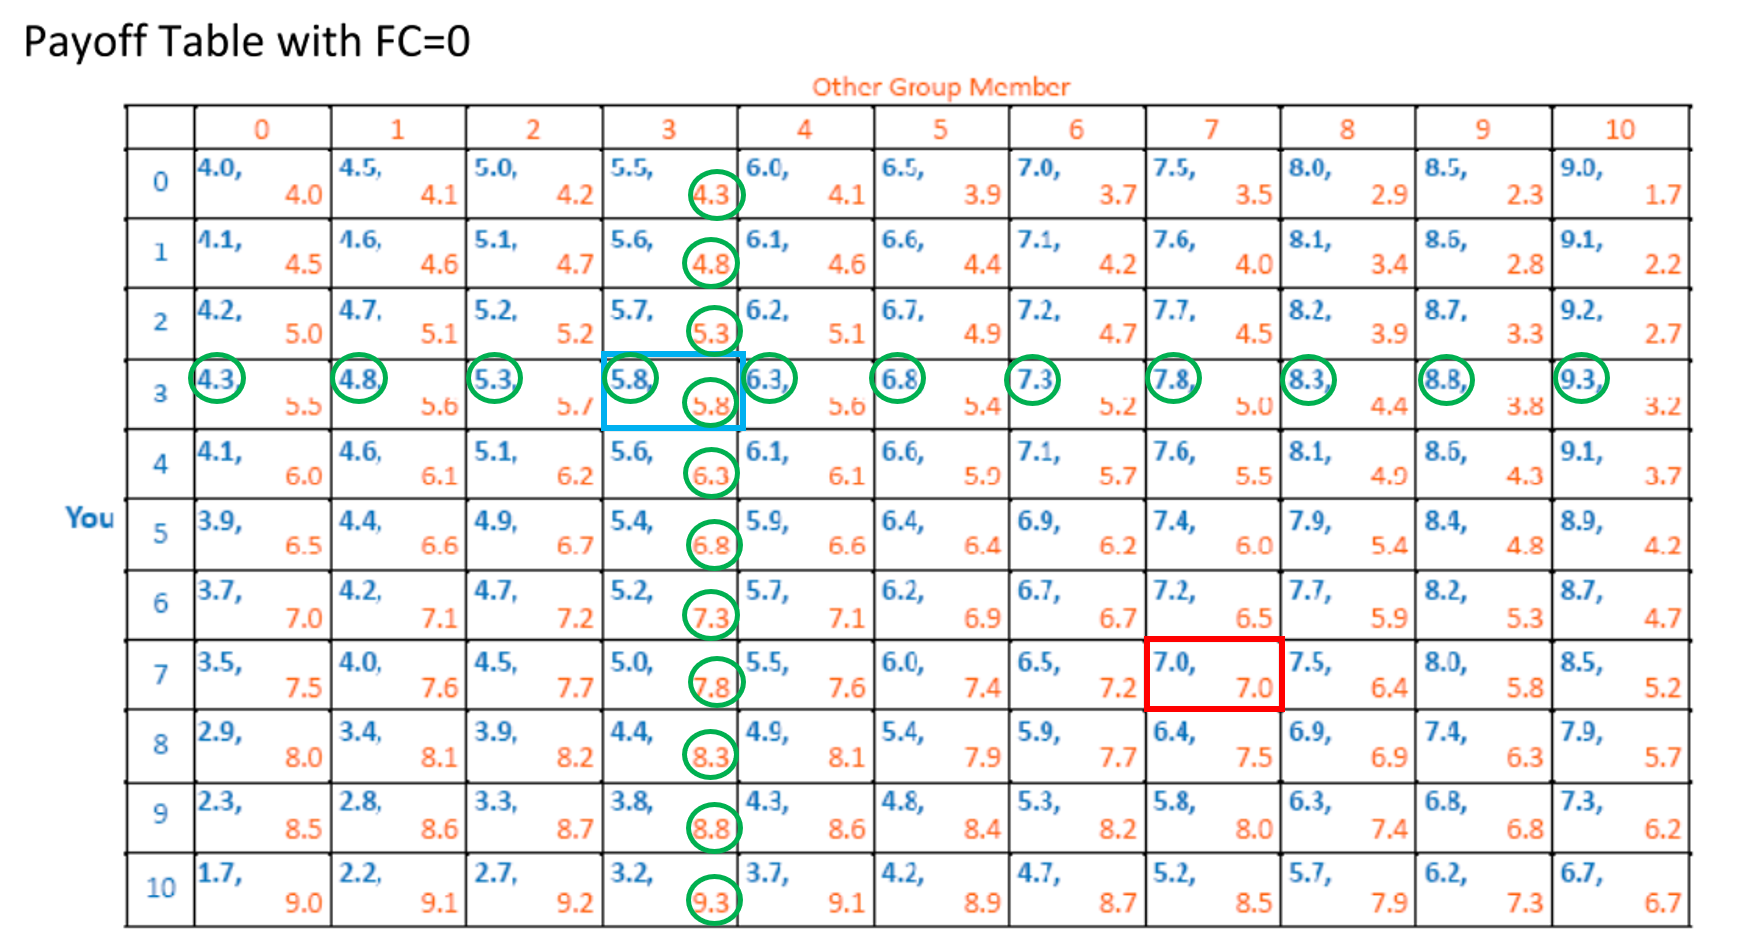
\includegraphics[width = 1.0\linewidth]{./0605kato_fig/payoff_FC0.png}}
    
    \end{frame}

    \begin{frame}
        \frametitle{Payoff Table with FC = 6}
    
        \centerline{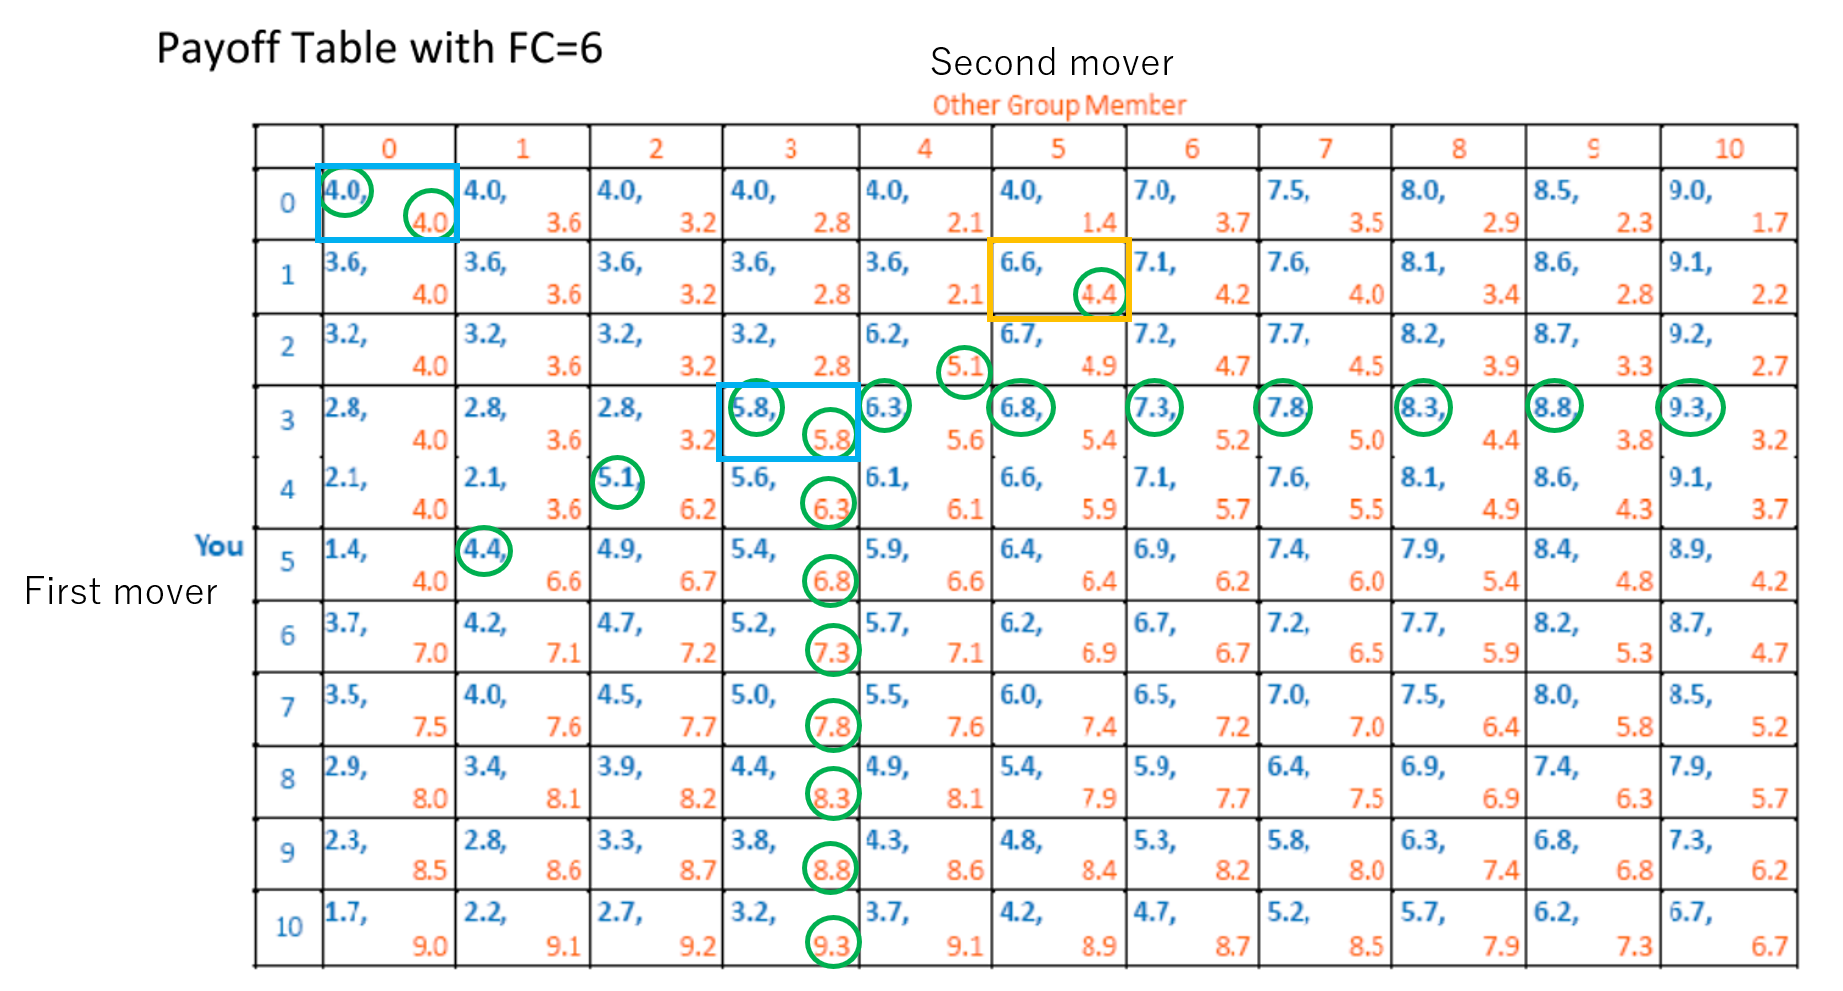
\includegraphics[width = 1.0\linewidth]{./0605kato_fig/payoff_FC6.png}}
    
    \end{frame}

    \begin{frame}
        \frametitle{Payoff Table with FC = 8}
    
        \centerline{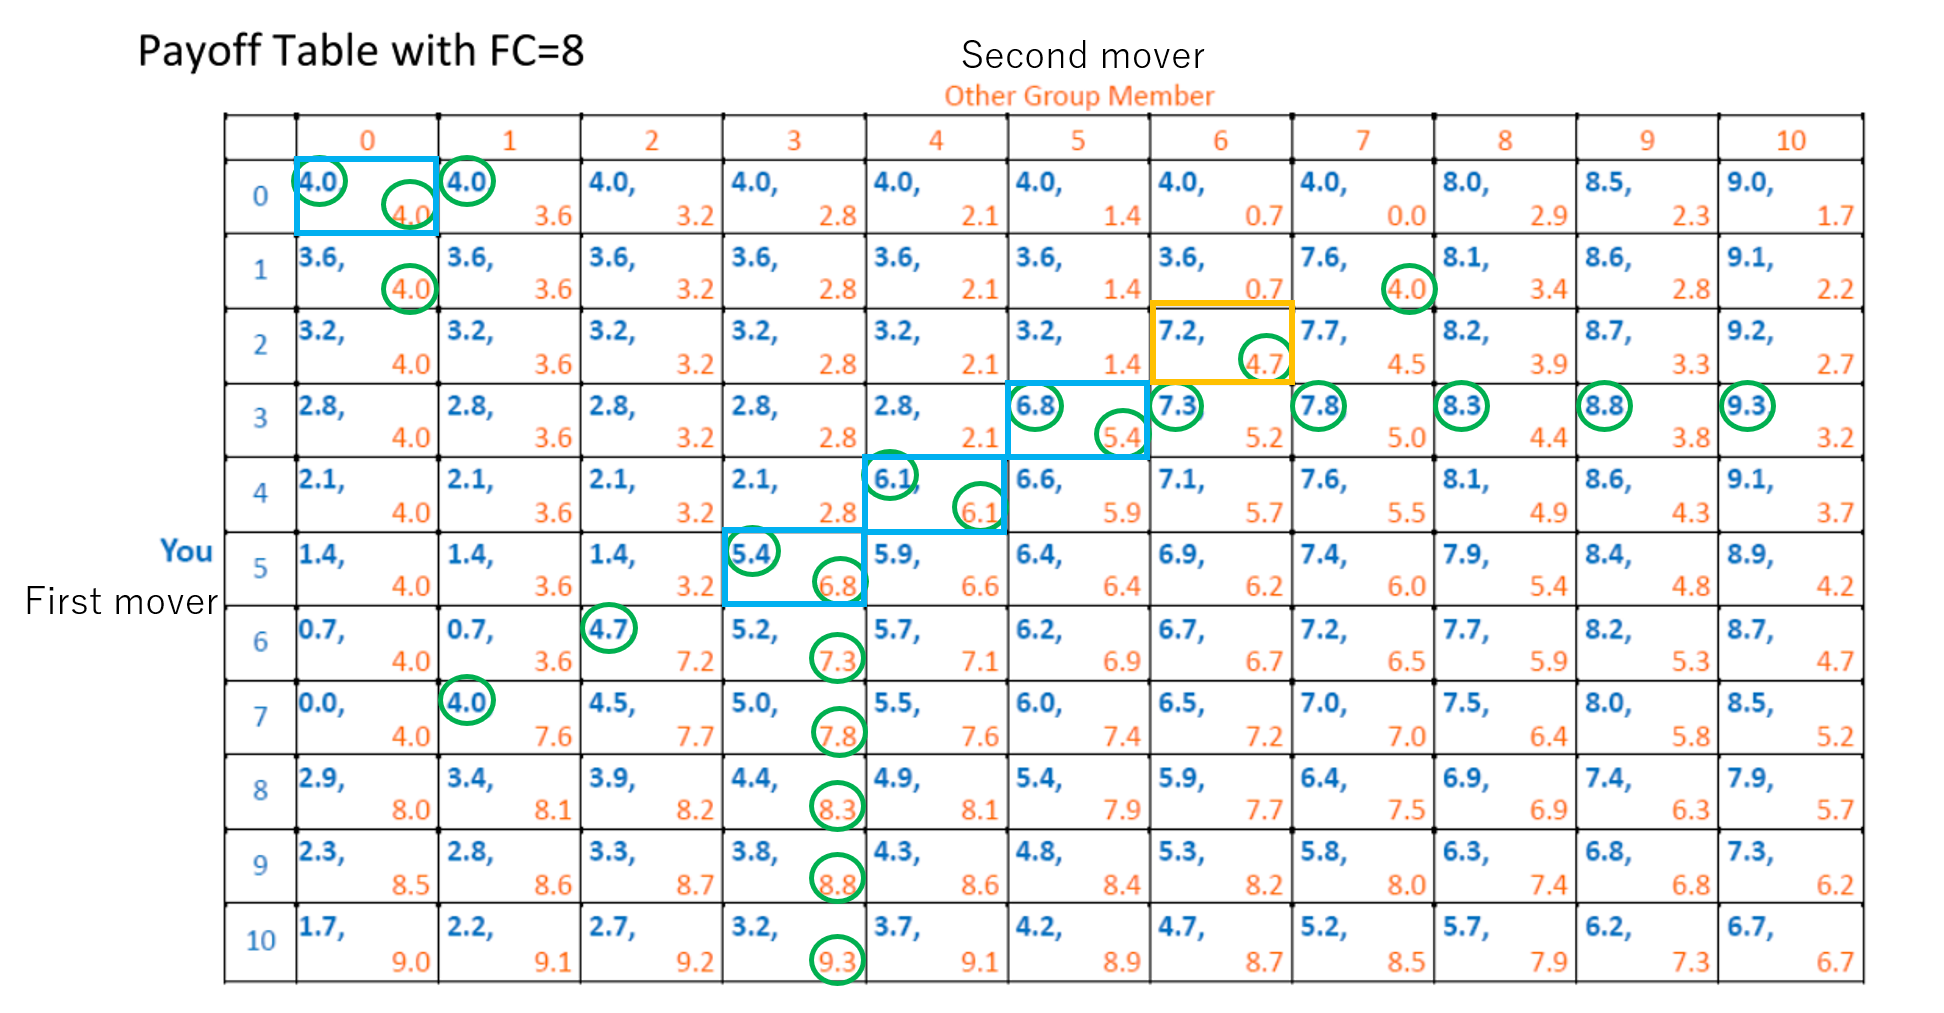
\includegraphics[width = 1.0\linewidth]{./0605kato_fig/payoff_FC8.png}}
    
    \end{frame}

    \begin{frame}
        \frametitle{Equlibrium Predictions}
    
        \begin{table}
            \centering
            \begin{tabular}{lccc}
                \hline
                &
                $FC = 0$ &
                $FC = 6$ &
                $FC = 8$ \\
                \hline 
                Sim &
                $\{(3,3)\}$ &
                $\{(0,0), (3,3)\}$ &
                $\{(0,0), (3,5), (4,4), (5,3)\}$ \\
                Seq &
                $\{(3,3)\}$ &
                $\{(1,5)\}$ &
                $\{(2,6)\}$ \\
                \hline
            \end{tabular}
        \end{table}
    
    \end{frame}

    \begin{frame}
        \frametitle{Procedure}
    
        \begin{itemize}
            \item Locate: the University of Pittsburgh.
            \item 224 undergraduate students (14 per session).
            \item Procedure:
            \begin{enumerate}
                \item Distributes instructions and payoff table
                \item A short quiz to gauge the participants' understanding.
                \item Distributes the solution key.
                \item Play 14 rounds of the public goods game. In each round, each participant was randomly paired with another participant.
            \end{enumerate}
            \item Payoff = (Random selected 3 rounds) + (\$5 show-up fee)
        \end{itemize}
    
    \end{frame}

    \section{Results}

    \begin{frame}
        \frametitle{Hypothesis 1}
    
        Without fixed costs, No effect of the sequential play on contributions
    
    \end{frame}

    \begin{frame}
        \frametitle{}
    
        \centerline{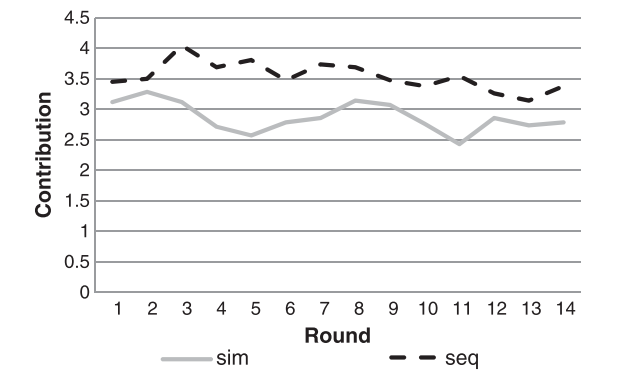
\includegraphics[width = 1.0\linewidth]{./0605kato_fig/h1.png}}
    
    \end{frame}

    \begin{frame}
        \frametitle{Result of Hypothesis 1}
    
        When fixed costs are zero, sequential play increases contributions
        \begin{itemize}
            \item A mean contribution of 2.87 units in the simultaneous game differs insignificantly from the prediction ($p = 0.382$).
            \item A mean contribution of 3.53 units in the sequential game differs significantly from the prediction ($p = 0.00$).
        \end{itemize}
    
    \end{frame}

    \begin{frame}
        \frametitle{Possible Explanation of Hypothesis 1}
    
        Reciprocity
        \begin{itemize}
            \item When the first mover's contribution ranges between 0 and 3 units, the average second mover contribution is 2.99 units.
            \item When the first mover's contribution is more than 3 units, the average second mover contribution is 3.80 units.
        \end{itemize}
    
    \end{frame}

    \begin{frame}
        \frametitle{Hypothesis 2}
    
        Mean contribution with 6 fixed costs are smaller than without fixed costs (simultaneous game)
    
    \end{frame}

    \begin{frame}
        \frametitle{}
    
        \centerline{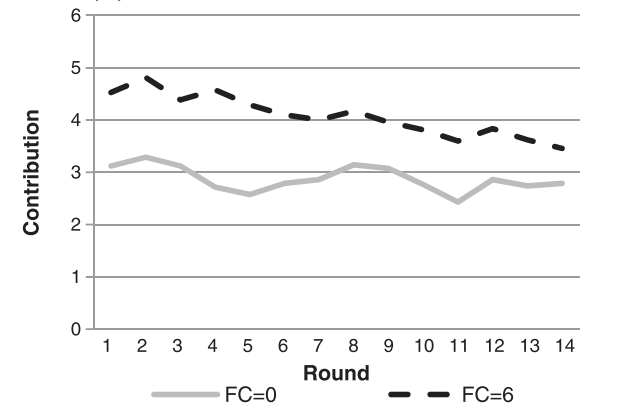
\includegraphics[width = 1.0\linewidth]{./0605kato_fig/h2.png}}
    
    \end{frame}

    \begin{frame}
        \frametitle{Result of Hypothesis 2}
    
        Reject hypothesis 2. the introduction of low fixed costs is found to significantly increase contributions rather than decreasing contributions.
        \begin{itemize}
            \item Regression shows that introducing a fixed cost of six increases individual contributions by 1.20 units all else equal.
        \end{itemize}
    
    \end{frame}

    \begin{frame}
        \frametitle{}
    
        \centerline{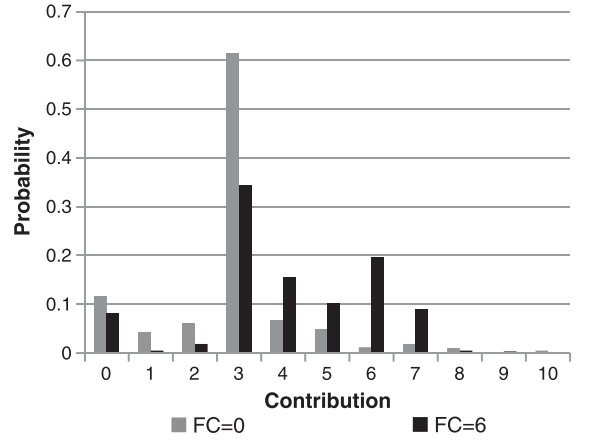
\includegraphics[width = 1.0\linewidth]{./0605kato_fig/h2_add.png}}
    
    \end{frame}

    \begin{frame}
        \frametitle{Possible Explanation of Hypotehsis 2}
    
        Strategic uncertainty
        \begin{itemize}
            \item Consider beliefs that only place weight on the partner selecting an action associated with the two Nash equilibria: 0 or 3 units.
            \item If the likelihood of being matched with a zero contributor lies in the range of 40 to 80\%, the best response is to contribute 6 units.
            \item Observe learning effect. During the first seven rounds, 3 and 6 unit contributions each account for 25\% of all play. These numbers change for the latter half of the experiment, with 44\% of all contributions at three and only 14\% at six.
        \end{itemize}
    
    \end{frame}

    \begin{frame}
        \frametitle{Hypothesis 3}
    
        Sequential play increases contributions with six fixed costs
    
    \end{frame}

    \begin{frame}
        \frametitle{}
    
        \centerline{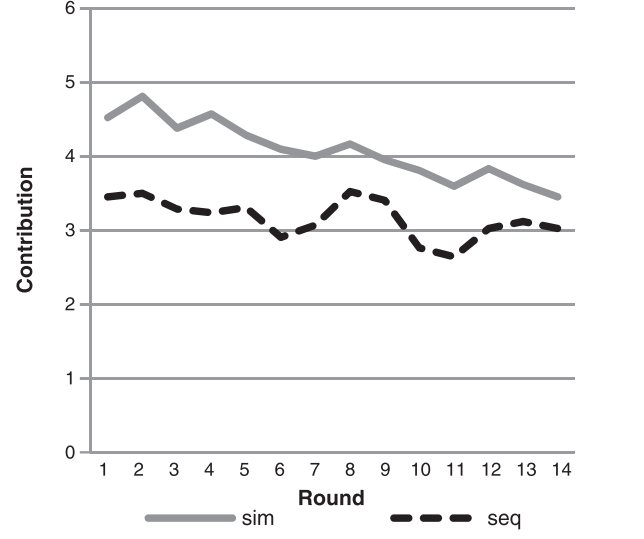
\includegraphics[width = 0.8\linewidth]{./0605kato_fig/h3.png}}
    
    \end{frame}

    \begin{frame}
        \frametitle{Result of Hypothesis 3}
    
        Reject hypothesis 3. With fixed costs of six, sequential play decreases the mean contribution.
        \begin{itemize}
            \item Regression result shows that sequential play reduces individual contributions by almost 1 unit all else equal.
            \item We cannot reject that the average contribution of 3.16 in the sequential game equals the predicted mean contribution, that is, 3 units ($p = 0.380$).
        \end{itemize}
        Possible explanation: A reduce of strategic uncertainty
    
    \end{frame}

    \begin{frame}
        \frametitle{}
    
        \centerline{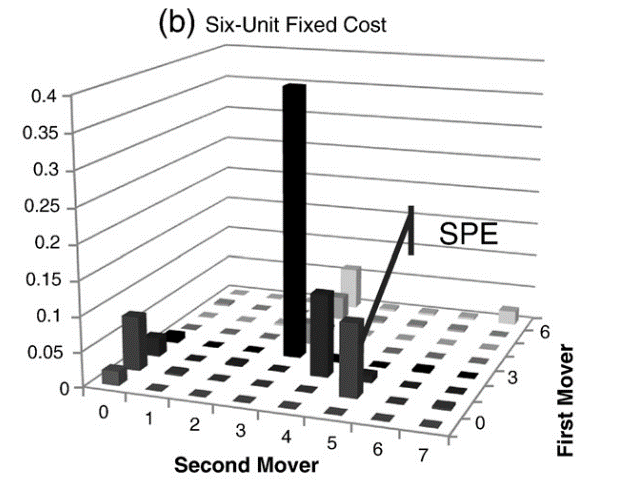
\includegraphics[width = 1.0\linewidth]{./0605kato_fig/eqm_FC6.png}}        
    
    \end{frame}

    \begin{frame}
        \frametitle{Equilibrium Selection with Low FC}
    
        \begin{itemize}
            \item Although provision rates are 86\%, participants shy away from the highlighted subgame perfect equilibrium $(1,5)$. The most common equilibrium is $(3,3)$.
            \item Thus, first movers cannot take advantage. Indeed, first movers earn 7 cents less than second movers, however this difference is not significant $(p = 0.60)$.
            \item Second movers may view contribution of one out of six as more unfair.
        \end{itemize}
    
    \end{frame}

    \begin{frame}
        \frametitle{Hypothesis 4}
    
        With an eight-unit fixed cost, sequential play increases contributions
    
    \end{frame}

    \begin{frame}
        \frametitle{}
    
        \centerline{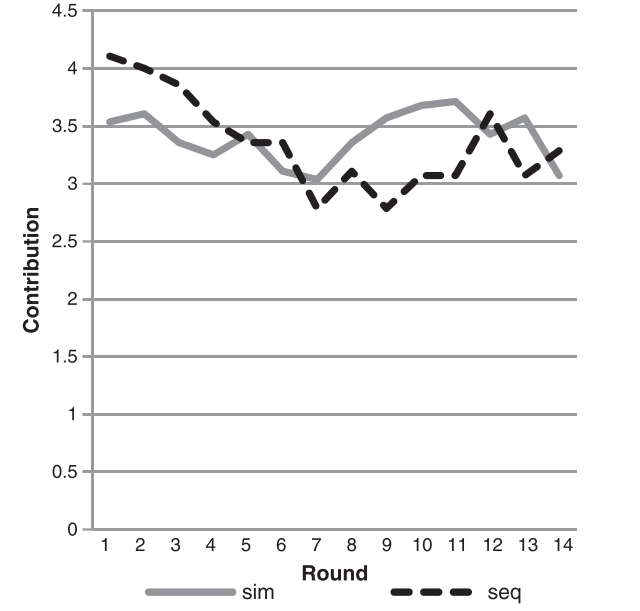
\includegraphics[width = 0.8\linewidth]{./0605kato_fig/h4.png}}
    
    \end{frame}


    \begin{frame}
        \frametitle{Result of Hypothesis 4}
    
        Reject hypothesis 4. Sequential play does not significantly increase individual contributions.
        However, \textit{sequential play increases round earnings by approximately \$1.20, a 27\% increase}.
        \begin{itemize}
            \item In the simultaneous game, a third of all contributions are at zero units.
            \item This result implies that the likelihood of providing the public good does increase substantially.
        \end{itemize}
    
    \end{frame}

    \begin{frame}
        \frametitle{}
    
        \centerline{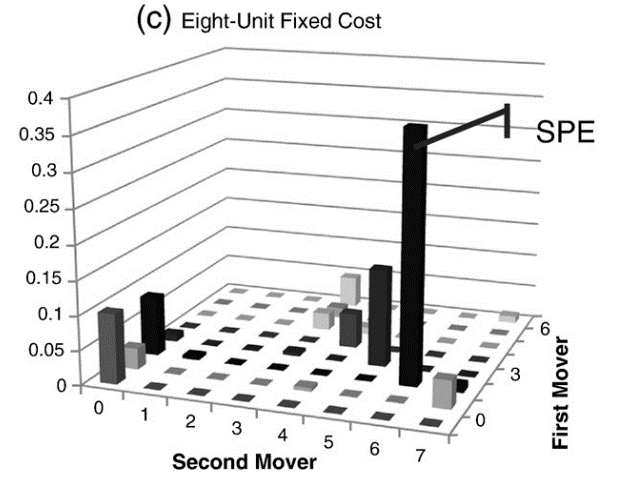
\includegraphics[width = 1.0\linewidth]{./0605kato_fig/eqm_FC8.png}}
            
    \end{frame}

    \begin{frame}
        \frametitle{Equlibrium Selection with High FC}
    
        \begin{itemize}
            \item Contrary to six units fixed costs, the most common equilibrium is the highlighted subgame perfect equilibrium of $(2,6)$.
            \item This leads to a significant and substantial first mover advantage. The earnings of first movers on average exceed those of the second movers by 87 cents. 
        \end{itemize}
    
    \end{frame}

    \section{Concluding Remarks}

    \begin{frame}
        \frametitle{Summary of Results}
    
        \begin{itemize}
            \item Behavior in both games is in line with the equilibrium predictions in the no and high fixed cost treatments.
            \item Behavior in both games is deviate from the predictions in the low fixed cost treatment.
            \begin{itemize}
                \item strategic uncertainty appears to cause greater than predicted simultaneous giving
                \item the tension associated with the substantial first mover advantage appears to move behavior away from the asymmetric subgame perfect equilibrium
            \end{itemize}
        \end{itemize}
    
    \end{frame}

    \begin{frame}
        \frametitle{Implications}
    
        \begin{quote}
            ..., the introduction of fixed costs increases the first mover advantage inherent in the public good game, and a potential risk of sequential play is that provision may fail unless the fundraiser is successful in convincing initial contributors to donate a fair share (p.426).
        \end{quote}
    
    \end{frame}


\end{document}